\documentclass[fsharpnotes.tex]{subfiles}
\graphicspath{ {./figures/} }

\begin{document}
\chapter{The Console in Windows,\\MacOS~X, and Linux}
\label{chap:console}
Almost all popular operating systems are accessed through a
user-friendly \idx{graphical user interface} (\idx{GUI}) that is designed to make typical tasks easy to learn to solve. As a computer programmer, you often need to access some of the functionalities of the computer, which, unfortunately, are sometimes complicated by this particular graphical user interface. The \idx{console}, also called the \idx{terminal} and the \idx{Windows command line}, is the right hand of a programmer. The console is a simple program that allows you to complete text commands. Almost all the tasks that can be done with the graphical user interface can be done in the console and vice versa. Using the console, you will benefit from its direct control of the programs we write, and in your education, you will benefit from the fast and raw information you get through the console.


\section{The Basics}
When you open a \idx{directory} or \idx{folder} in your preferred operating system, the directory will have a location in the file system, whether from the console or through the operating system's graphical user interface. The console will almost always be associated with a particular directory or folder in the file system, and it is said that it is the directory that the console is in. The exact structure of file systems varies between Linux, MacOS X, and Windows, but common is that it is a hierarchical structure. This is illustrated in \Cref{fig:filhierakier}.
\begin{figure}
  \begin{center}
  \subfigure[Linux]{\Tree [.\framebox{/} [.\framebox{home} [. {\framebox{Username}} ] ] {\framebox{usr}} {\framebox{bin}} {\framebox{dev}} {\framebox{...}} ]}
  \subfigure[MacOS X]{\Tree [.\framebox{/} [.\framebox{Users} [. {\framebox{Username}} ] ] {\framebox{usr}} {\framebox{bin}} {\framebox{dev}} {\framebox{etc}} ]}
  \subfigure[Windows]{\Tree [.\framebox{C:\textbackslash} [.\framebox{Users} [. {\framebox{Username}} ] ] {\framebox{Program Files}} {\framebox{Program Files (x86)}} {\framebox{...}} ]}
    % \scalebox{0.23}
   % {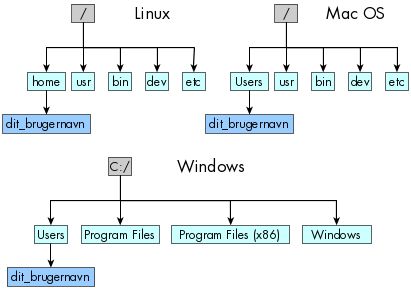
\includegraphics[width=\textwidth]{filehira.png}}
  \end{center}
  \caption{The top file hierarchy levels of common operating systems.}
  \label{fig:filhierakier}
\end{figure}

There are many predefined console commands, available in the console, and you can also make your own. In the following sections, we will review the most important commands in the three different operating systems. These are summarized in \Cref{tab:Kommandoer}.
\begin{table}
  \centering
  \rowcolors{2}{oddRowColor}{evenRowColor}
  \begin{tabularx}{\linewidth}{|l|l|>{\raggedright\arraybackslash}X|}
    \hline
    Windows & MacOS X/Linux & Description 
    \\ \hline\hline
    {\lstinline[language=syntax]!d!}
            & {\lstinline[language=syntax]!ls!}
                            & Show content of present directory.
    \\ \hline
    {\lstinline[language=syntax]!cd <*d*>!} 
            &{\lstinline[language=syntax]!cd <*d*>!} 
                          & Change present directory to {\lstinline[language=syntax]!<*d*>!}. 
    \\ \hline
    % {\lstinline[language=syntax]!touch <*fil*>!} & opret en tom fil med navnet {\lstinline[language=syntax]!<*fil*>!}. \\ \hline
    %{\lstinline[language=syntax]!emacs <*fil*>!}
    %         & Åben {\lstinline[language=syntax]!<*fil*>!} i emacs hvis den findes i den nuværende mappe. Findes den ikke oprettes den her automatisk.   \\ \hline
    {\lstinline[language=syntax]!mkdir <*d*>!}
            & {\lstinline[language=syntax]!mkdir <*d*>!}
                          & Create directory {\lstinline[language=syntax]!<*d*>!}. \\ \hline
    {\lstinline[language=syntax]!rmdir <*d*>!}
            & {\lstinline[language=syntax]!rmdir <*d*>!}
                          & Delete {\lstinline[language=syntax]!<*d*>!} (Warning: cannot be reverted). \\ \hline
    {\lstinline[language=syntax, keywords={}]!move <*f*> <*f | d*>!\hspace*{5mm}}% The gobling of <**> causes spacing problems...
            &{\lstinline[language=syntax, keywords={}]!mv <*f*> <*f | d*>!}
                          & Move {\lstinline[language=syntax]!<*fil*>!} to {\lstinline[language=syntax, keywords={}]!<*f | d*>!}. \\ \hline
    {\lstinline[language=syntax]!copy <*f1*> <*f2*>!}
            &{\lstinline[language=syntax]!cp <*f1*> <*f2*>!}
             & Create a new file called {\lstinline[language=syntax]!<*f2*>!} as a copy of {\lstinline[language=syntax]!<*f1*>!}. \\ \hline
    {\lstinline[language=syntax]!del <*f*>!}
            & {\lstinline[language=syntax]!rm <*f*>!}
                          & delete {\lstinline[language=syntax]!<*f*>!} (Warning: cannot be reverted). \\ \hline
    {\lstinline[language=syntax, keywords={}]!echo <*s | v*>!\hspace*{5mm}}
            & {\lstinline[language=syntax, keywords={}]!echo <*s | v*>!\hspace*{5mm}}
                          & Write a string or content of a variable to screen. \\ \hline
  \end{tabularx}\\
  \caption{The most important console commands for Windows, MacOS X,
    and Linux. Here \lstinline[language=syntax]{<*f**>} is shorthand for any filename,
  \lstinline[language=syntax]{<*d*>} for any directory name,
\lstinline[language=syntax]{<*s*>} for any string, and
\lstinline[language=syntax]{<*v*>} for any shell-variable.}
  \label{tab:Kommandoer}
\end{table}


\section{Windows}
In this section we will discuss the commands summarized in \Cref{tab:Kommandoer}. Windows 7 and earlier versions: To open the console, press \lstinline[language=console]{Start->Run} in the lower left corner, and then type \lstinline[language=console]{cmd} in the box. In Windows 8 and 10, you right-click on the windows icon, choose \lstinline[language=console]{Run} or equivalent in your local language, and type \lstinline[language=console]{cmd}. Alternatively, you can type \lstinline[language=console]{Windows-key + R}. Now you should open a console window with a prompt showing something like \Cref{windowsConsole}.
\begin{codeNOutput}[label=windowsConsole]{: The Windows console.}
  \begin{lstlisting}[language=console,escapechar=§]
Microsoft Windows [Version 6.1.7601]
Copyright (c) 2009 Microsoft Corporation.  All rights reserved.

C:\Users\sporring>
\end{lstlisting}
\end{codeNOutput}
To see which files are in the directory, use \idx[dir@{\lstinline[language=console]{dir}}]{\lstinline[language=console]{dir}}, as shown in \Cref{windowsDir}.
\begin{codeNOutput}[label=windowsDir]{: Directory listing with \lstinline[language=console]{dir}.}
  \begin{lstlisting}[language=console,escapechar=§]
C:\Users\sporring>dir
 Volume in drive C has no label.
 Volume Serial Number is 94F0-31BD

 Directory of C:\Users\sporring

30-07-2015  15:23    <DIR>          .
30-07-2015  15:23    <DIR>          ..
30-07-2015  14:27    <DIR>          Contacts
30-07-2015  14:27    <DIR>          Desktop
30-07-2015  17:40    <DIR>          Documents
30-07-2015  15:11    <DIR>          Downloads
30-07-2015  14:28    <DIR>          Favorites
30-07-2015  14:27    <DIR>          Links
30-07-2015  14:27    <DIR>          Music
30-07-2015  14:27    <DIR>          Pictures
30-07-2015  14:27    <DIR>          Saved Games
30-07-2015  17:27    <DIR>          Searches
30-07-2015  14:27    <DIR>          Videos
               0 File(s)              0 bytes
              13 Dir(s)  95.004.622.848 bytes free

C:\Users\sporring>
\end{lstlisting}
\end{codeNOutput}
We see that there are no files and thirteen directories (DIR). The columns tell from left to right: the date and time of their creation, the file size or if it is a folder, and the name file or directory name. The first two folders ``\lstinline[language=console]{.}'' and ``\lstinline[language=console]{..}'' are found in each folder and refer to this folder as well as the one above in the hierarchy. In this case, the folder ``\lstinline[language=console]{.}'' is an alias for \lstinline[language=console]{C:\Users\sporring} and ``\lstinline[language=console]{..}'' for \lstinline[language=console]{C:\Users}.

Use \idx[cd@{\lstinline[language=console]{cd}}]{\lstinline[language=console]{cd}} to change directory, e.g.,  to \lstinline[language=console]{Documents}, as in \Cref{windowsCD}.
\begin{codeNOutput}[label=windowsCD]{: Change directory with \lstinline[language=console]{cd}.}
  \begin{lstlisting}[language=console,escapechar=§]
C:\Users\sporring>cd Documents

C:\Users\sporring\Documents>
\end{lstlisting}
\end{codeNOutput}
Note that some systems translate default filenames, so their names may be given different names in different languages in the graphical user interface as compared to the console. 

% On a new computer is the \lstinline[language=console]{Documents} folder is typically empty, as shown in \Cref{windowsDirEmpty}.
% \begin{codeNOutput}[label=windowsDirEmpty]{: A new directory is always empty.}
%   \begin{lstlisting}[language=console,escapechar=§]
% C:\Users\sporring\Documents>dir
%  Volume in drive C has no label.
%  Volume Serial Number is 94F0-31BD

%  Directory of C:\Users\sporring\Documents

% 30-07-2015  19:16    <DIR>          .
% 30-07-2015  19:16    <DIR>          ..
%                0 File(s)              0 bytes
%                2 Dir(s)  94.656.716.800 bytes free

% C:\Users\sporring\Documents>
% \end{lstlisting}
% \end{codeNOutput}
You can use \idx[mkdir@{\lstinline[language=console]{mkdir}}]{\lstinline[language=console]{mkdir}} to create a new directory called, e.g., \lstinline[language=console]{myFolder}, as illustrated in \Cref{windowsMkdir}.
\begin{codeNOutput}[label=windowsMkdir]{: Creating a directory with \lstinline[language=console]{mkdir}.}
  \begin{lstlisting}[language=console,escapechar=§]
C:\Users\sporring\Documents>mkdir myFolder

C:\Users\sporring\Documents>dir
 Volume in drive C has no label.
 Volume Serial Number is 94F0-31BD

 Directory of C:\Users\sporring\Documents

30-07-2015  19:17    <DIR>          .
30-07-2015  19:17    <DIR>          ..
30-07-2015  19:17    <DIR>          myFolder
               0 File(s)              0 bytes
               3 Dir(s)  94.656.638.976 bytes free

C:\Users\sporring\Documents>
\end{lstlisting}
\end{codeNOutput}
By using \lstinline[language=console]{dir} we inspect the result.

Files can be created by, e.g., \idx[echo@{\lstinline[language=console]{echo}}]{\lstinline[language=console]{echo}} and \idx{redirection}, as demonstrated in \Cref{windowsEcho}.
\begin{codeNOutput}[label=windowsEcho]{: Creating a file with \lstinline[language=console]{echo} and redirection.}
  \begin{lstlisting}[language=console,escapechar=§]
C:\Users\sporring\Documents>echo "Hi" > hi.txt

C:\Users\sporring\Documents>dir
 Volume in drive C has no label.
 Volume Serial Number is 94F0-31BD

 Directory of C:\Users\sporring\Documents

30-07-2015  19:18    <DIR>          .
30-07-2015  19:18    <DIR>          ..
30-07-2015  19:17    <DIR>          myFolder
30-07-2015  19:18                 8 hi.txt
               1 File(s)              8 bytes
               3 Dir(s)  94.656.634.880 bytes free

C:\Users\sporring\Documents>
\end{lstlisting}
\end{codeNOutput}
To move the file \lstinline[language=console]{hi.txt} to the directory \lstinline[language=console]{myFolder}, use \idx[move@{\lstinline[language=console]{move}}]{\lstinline[language=console]{move}}, as shown in \Cref{windowsMove}.
\begin{codeNOutput}[label=windowsMove]{: Move a file with \lstinline[language=console]{move}.}
  \begin{lstlisting}[language=console,escapechar=§]
C:\Users\sporring\Documents>move hi.txt myFolder
        1 file(s) moved.

C:\Users\sporring\Documents>
\end{lstlisting}
\end{codeNOutput}
Finally, use \idx[del@{\lstinline[language=console]{del}}]{\lstinline[language=console]{del}} to delete a file and \idx[rmdir@{\lstinline[language=console]{rmdir}}]{\lstinline[language=console]{rmdir}} to delete a directory, as shown in \Cref{windowsDel}.
\begin{codeNOutput}[label=windowsDel]{: Delete files and directories with \lstinline[language=console]{del} and \lstinline[language=console]{rmdir}.}
  \begin{lstlisting}[language=console,escapechar=§]
C:\Users\sporring\Documents>cd myFolder

C:\Users\sporring\Documents\myFolder>del hi.txt

C:\Users\sporring\Documents\myFolder>cd ..

C:\Users\sporring\Documents>rmdir myFolder

C:\Users\sporring\Documents>dir
 Volume in drive C has no label.
 Volume Serial Number is 94F0-31BD

 Directory of C:\Users\sporring\Documents

30-07-2015  19:20    <DIR>          .
30-07-2015  19:20    <DIR>          ..
               0 File(s)              0 bytes
               2 Dir(s)  94.651.142.144 bytes free

C:\Users\sporring\Documents>
\end{lstlisting}
\end{codeNOutput}
The commands available from the console must be in its \idx{search path}. The search path can be seen using \lstinline[language=console]{echo}, as shown in \Cref{windowsPath}.
\begin{codeNOutput}[label=windowsPath]{: Displaying the search path.}
  \begin{lstlisting}[language=console,escapechar=§]
C:\Users\sporring\Documents>echo %Path%
C:\Windows\system32;C:\Windows;C:\Windows\System32\Wbem; C:\Windows\System32\WindowsPowerShell\v1.0\;"\Program Files\emacs-24.5\bin\"

C:\Users\sporring\Documents>
\end{lstlisting}
\end{codeNOutput}
The path can be changed using the Control panel in the graphical user interface. In Windows 7, choose the Control panel, choose \lstinline[language=console]{System and Security} $\rightarrow$ \lstinline[language=console]{System} $\rightarrow$ \lstinline[language=console]{Advanced system settings} $\rightarrow$ \lstinline[language=console]{Environment Variables}. In Windows 10, you can find this window by searching for ``Environment'' in the Control panel. In the window's \lstinline[language=console]{System variables} box, double-click on \lstinline[language=console]{Path} and add or remove a path from the list. The search path is a list of paths separated by ``;''. Beware, Windows uses the search path for many different tasks, so remove only paths that you are certain are not used for anything.

A useful feature of the console is that you can use the \lstinline[language=console]{tab}-key to cycle through filenames.  E.g., if you write \lstinline[language=console]{cd} followed by a space and \lstinline[language=console]{tab} a couple of times, then the console will suggest to you the available directories.

\section{MacOS X and Linux}
MacOS X (OSX) and Linux are very similar, and both have the option of using \idx[bash@{\lstinline[language=console]{bash}}]{\lstinline[language=console]{bash}} as console. It is in the standard console on MacOS X and on many Linux distributions. A summary of the most important \lstinline[language=console]{bash} commands is shown in \Cref{tab:Kommandoer}. In MacOS X, you find the console by opening \lstinline[language=console]{Finder} and navigating to \lstinline[language=console]{Applications} $\rightarrow$ \lstinline[language=console]{Utilities} -> \lstinline[language=console]{Terminal}.  In Linux, the console can be started by typing \lstinline[language=console]{Ctrl + Alt + T}. Some Linux distributions have other key-combinations such as \lstinline[language=console]{Super + T}. 

Once opened, the console is shown in a window with content, as shown in \Cref{LinuxConsole}.
\begin{codeNOutput}[label=LinuxConsole]{: The MacOS console.}
  \begin{lstlisting}[language=console,escapechar=§]
Last login: Thu Jul 30 11:52:07 on ttys000
FN11194:~ sporring$ 
\end{lstlisting}%$
\end{codeNOutput}
``FN11194'' is the name of the computer, the character $\sim$ is used as an alias for the user's home directory, and ``sporring'' is the username for the user presently logged onto the system. Use \idx[ls@{\lstinline[language=console]{ls}}]{\lstinline[language=console]{ls}} to see which files are present, as shown in \Cref{LinuxLs}.
\begin{codeNOutput}[label=LinuxLs]{: Display a directory content with \lstinline[language=console]{ls}.}
  \begin{lstlisting}[language=console,escapechar=§]
FN11194:~ sporring$ ls
Applications    Documents    Library        Music        Public
Desktop        Downloads    Movies        Pictures
FN11194:~ sporring$ 
\end{lstlisting}
\end{codeNOutput}
More details about the files are available by using flags to \lstinline[language=console]{ls} as demonstrated in \Cref{LinuxLsFlags}.
\begin{codeNOutput}[label=LinuxLsFlags]{: Display extra information about files using flags to \lstinline[language=console]{ls}.}
  \begin{lstlisting}[language=console,escapechar=§]
FN11194:~ sporring$ ls -l
drwx------   6 sporring  staff   204 Jul 30 14:07 Applications
drwx------+ 32 sporring  staff  1088 Jul 30 14:34 Desktop
drwx------+ 76 sporring  staff  2584 Jul  2 15:53 Documents
drwx------+  4 sporring  staff   136 Jul 30 14:35 Downloads
drwx------@ 63 sporring  staff  2142 Jul 30 14:07 Library
drwx------+  3 sporring  staff   102 Jun 29 21:48 Movies
drwx------+  4 sporring  staff   136 Jul  4 17:40 Music
drwx------+  3 sporring  staff   102 Jun 29 21:48 Pictures
drwxr-xr-x+  5 sporring  staff   170 Jun 29 21:48 Public
FN11194:~ sporring$ 
\end{lstlisting}
\end{codeNOutput}
The flag \lstinline[language=console]{-l} means long, and many other flags can be found by querying the built-in manual with \lstinline[language=console]{man ls}. The output is divided into columns, where the left column shows a number of codes:  ``d'' stands for directory, and the set of three of optional ``rwx'' denote whether respectively the owner, the associated group of users, and anyone can respectively ``r'' - read, ``w'' - write, and ``x'' - execute the file. In all directories but the \lstinline[language=console]{Public} directory, only the owner can do any of the three. For directories, ``x'' means permission to enter. The second column can often be ignored, but shows how many links there are to the file or directory. Then follows the username of the owner, which in this case is \lstinline[language=console]{sporring}. The files are also associated with a group of users, and in this case, they all are associated with the group called \lstinline[language=console]{staff}. Then follows the file or directory size, the date of last change, and the file or directory name. There are always two hidden directories: ``\lstinline[language=console]{.}'' and ``\lstinline[language=console]{..}'', where ``\lstinline[language=console]{.}'' is an alias for the present directory, and ``\lstinline[language=console]{..}'' for the directory above. Hidden files will be shown with the \lstinline[language=console]{-a} flag.

Use \idx[cd@{\lstinline[language=console]{cd}}]{\lstinline[language=console]{cd}} to change to the directory, for example to \lstinline[language=console]{Documents} as shown in \Cref{LinuxCd}.
\begin{codeNOutput}[label=LinuxCd]{: Change directory with \lstinline[language=console]{cd}.}
  \begin{lstlisting}[language=console,escapechar=§]
FN11194:~ sporring$ cd Documents/
FN11194:Documents sporring$ 
\end{lstlisting}
\end{codeNOutput}
Note that some graphical user interfaces translate standard filenames and directories to the local language, such that navigating using the graphical user interface will reveal other files and directories, which, however, are aliases. 

%On a new computer many directories are predefined but empty
% , e.g., \lstinline[language=console]{Documents} as shown in \Cref{LinuxEmpty}.
% \begin{codeNOutput}[label=LinuxEmpty]{: New directories are empty.}
%   \begin{lstlisting}[language=console,escapechar=§]
% FN11194:Documents sporring$ ls
% FN11194:Documents sporring$  
% \end{lstlisting}
% \end{codeNOutput}
You can create a new directory using \idx[mkdir@{\lstinline[language=console]{mkdir}}]{\lstinline[language=console]{mkdir}}, as demonstrated in \Cref{LinuxMkdir}.
\begin{codeNOutput}[label=LinuxMkdir]{: Creating a directory using \lstinline[language=console]{mkdir}.}
  \begin{lstlisting}[language=console,escapechar=§]
FN11194:Documents sporring$  mkdir myFolder
FN11194:Documents sporring$ ls
myFolder
FN11194:tmp sporring$  
\end{lstlisting}%$
\end{codeNOutput}
A file can be created using \idx[echo@{\lstinline[language=console]{echo}}]{\lstinline[language=console]{echo}} and with \idx{redirection}, as shown in \Cref{LinuxEcho}.
\begin{codeNOutput}[label=LinuxEcho]{: Creating a file with \lstinline[language=console]{echo} and redirection.}
  \begin{lstlisting}[language=console,escapechar=§]
FN11194:Documents sporring$ echo "hi" > hi.txt
FN11194:Documents sporring$ ls
hi.txt        myFolder
\end{lstlisting}
\end{codeNOutput}
To move the file \lstinline[language=console]{hi.txt} into \lstinline[language=console]{myFolder}, use \idx[mv@{\lstinline[language=console]{mv}}]{\lstinline[language=console]{mv}}. This is demonstrated in \Cref{LinuxMv}.
\begin{codeNOutput}[label=LinuxMv]{: Moving files with \lstinline[language=console]{mv}.}
  \begin{lstlisting}[language=console,escapechar=§]
FN11194:Documents sporring$ echo mv hi.txt myFolder/
FN11194:Documents sporring$ 
\end{lstlisting}
\end{codeNOutput}
To delete the file and the directory, use \idx[rm@{\lstinline[language=console]{rm}}]{\lstinline[language=console]{rm}}  and \idx[rmdir@{\lstinline[language=console]{rmdir}}]{\lstinline[language=console]{rmdir}}, as shown in \Cref{LinuxRm}.
\begin{codeNOutput}[label=LinuxRm]{: Deleting files and directories.}
  \begin{lstlisting}[language=console,escapechar=§]
FN11194:Documents sporring$ cd myFolder/
FN11194:myFolder sporring$ rm hi.txt 
FN11194:myFolder sporring$ cd ..
FN11194:Documents sporring$ rmdir myFolder/
FN11194:Documents sporring$ ls
FN11194:Documents sporring$ 
\end{lstlisting}
\end{codeNOutput}
Only commands found on the \idx{search path} are available in the console. The content of the search path is seen using the \lstinline[language=console]{echo} command, as demonstrated in \Cref{LinuxSearchPath}.
\begin{codeNOutput}[label=LinuxSearchPath]{: The content of the search path.}
  \begin{lstlisting}[language=console,escapechar=§]
FN11194:Documents sporring$ echo $PATH
/Applications/Maple 17/:/Applications/PackageMaker.app/Contents/MacOS/: /Applications/MATLAB_R2014b.app/bin/:/opt/local/bin: /opt/local/sbin:/usr/local/bin:/usr/bin:/bin:/usr/sbin: /sbin:/opt/X11/bin:/Library/TeX/texbin
FN11194:Documents sporring$ 
\end{lstlisting}%$
\end{codeNOutput}
The search path can be changed by editing the setup file for Bash. On MacOS X it is called \lstinline[language=console]{~/.profile}, and on Linux it is either \lstinline[language=console]{~/.bash_profile} or \lstinline[language=console]{~/.bashrc}. Here new paths can be added by adding the following line: \lstinline[language=console]{export PATH="<new path>:<another new path>:$PATH"}. %$

A useful feature of Bash is that the console can help you write commands. E.g., if you write \lstinline[language=console]{fs} followed by pressing the \lstinline[language=console]{tab}-key, and if Mono is in the search path, then Bash will typically respond by completing the line as \lstinline[language=console]{fsharp}, and by further pressing the \lstinline[language=console]{tab}-key some times, Bash will show the list of options, typically \lstinline[language=console]{fshpari} and \lstinline[language=console]{fsharpc}. Also, most commands have an extensive manual which can be accessed using the \lstinline[language=console]{man} command. E.g., the manual for \lstinline[language=console]{rm} is retrieved by \lstinline[language=console]{man rm}.
\end{document}
